\documentclass[a4paper,12pt]{article}
    \usepackage[acronym,toc]{glossaries}
    \usepackage{graphicx} % For figures later
    \usepackage[utf8]{inputenc}
    \usepackage{mathptmx}
    \usepackage{titling}
    \usepackage{comment}
    \graphicspath{ {../images/} }
    \usepackage{caption}
    % SQL tables
    \usepackage{listings}
    \usepackage{float}
    \usepackage{enumerate}% http://ctan.org/pkg/enumerate
    \usepackage[titletoc]{appendix}
    \usepackage{array}
    \newcolumntype{L}[1]{>{\raggedright\let\newline\\\arraybackslash\hspace{0pt}}m{#1}}
    \newcolumntype{C}[1]{>{\centering\let\newline\\\arraybackslash\hspace{0pt}}m{#1}}
    \newcolumntype{R}[1]{>{\raggedleft\let\newline\\\arraybackslash\hspace{0pt}}m{#1}}
    \usepackage{tikz}
    \def\checkmark{\tikz\fill[scale=0.4](0,.35) -- (.25,0) -- (1,.7) -- (.25,.15) -- cycle;} 
    
    
    \makeglossaries
    
    \newglossaryentry{mysql}
    {
        name=MySQL,
        description={ is an open-source relational database management system }
    } 
    \newglossaryentry{docker}
    {
        name=Docker,
        description={  Docker provides an additional layer of abstraction and automation of operating-system-level virtualization on Windows, Linux and MacOS }
    }  
    \newglossaryentry{scala}
    {
        name=Scala,
        description={ Scala is a general-purpose programming language providing support for functional programming and a strong static type system }
    }   
	 \newglossaryentry{seimas}
	{
		name=Seimas,
		description={ The Seimas of the Republic of Lithuania, or simply the Seimas is the unicameral parliament of Lithuania. The Seimas constitutes the legislative branch of government in Lithuania, enacting laws and amendments to the Constitution, passing the budget, confirming the Prime Minister and the Government and controlling their activities }
	} 
   \newglossaryentry{lrs_open}
	{
		name=LRS open data,
		description={ Open data of Lietuvos Respublikos Seimas}
	}   
   \newglossaryentry{k-means}
	{
		name=\textit{k-means},
		description={ }
	} 
   \newglossaryentry{dissimilarity_matrix}
	{
		name=dissimilarity matrix,
		description={ }
	} 
   \newglossaryentry{atviras_seimas}
	{
		name=atviras-seimas.lt,
		description={ }
	} 



    
    % TODO check this list
    \newacronym{api}{API}{Application programming interface}
    \newacronym{auc}{AUC}{ Area under the curve }
    \newacronym{roc}{ROC}{ Receiver operating characteristic }
    \newacronym{hdd}{HDD}{ Hard disk drive }
    \newacronym{csv}{CSV}{ Comma-separated values}
    \newacronym{ip}{IP}{ Internet protocol address }
    \newacronym{tfidf}{TFIDF}{ Term Frequency Inverse Document Frequency }
    \newacronym{io}{IO}{ Input/Output }
    \newacronym{mds}{MDS}{ Multidimensional scaling}
    \newacronym{lrs}{LRS}{ Parliament of the Republic of Lithuania } 
    \newacronym{xml}{XML}{ PLACEHOLDER }   
    
    \begin{document}
   
    
    \pagenumbering{roman}
    
    \begin{center}
        \section*{Abstract}
    \end{center}
        
        \addcontentsline{toc}{section}{\numberline{}\kern-1.5emAbstract}%
        
%         \title{{\vspace{-4cm} \large Lithuanian parliament legislative voting analysis and vizualization} \vspace{-1cm}}
%         \author{\small Author: Žygimantas Benetis\\\small Supervisor: Prof. Dr. Tomas Krilavičius}
%         \maketitle
        
        In Republic of Lithuania, public elects their representatives to a parliament in which new legislation is considered. Due nature of politics, a problem arises once citizens wants to observe and evaluate parliament members work. Main output of parliament is their votes for various legislatures. Voting data is publicly available through \gls{lrs} website. This project aims to visualize voting patterns and their changes. Another goal is to provide public access to results.
        
        In the project \gls{mds} and \gls{k-means} clustering are used to analyze voting patterns. Software to download, process and visualize  data is written with \gls{scala}.
        
        
        
    \clearpage
    
    \tableofcontents
    
    \clearpage
    
    \printglossary[type=\acronymtype]
    
    \clearpage
    
    \printglossary
    
    \clearpage
    
    \pagenumbering{arabic}
    
    \section{Introduction}
    
    In Republic of Lithuania, public elects their representatives to a parliament in which new legislation is considered. By this election each citizen delegates specifics of legislation process to their representatives so they don't have to actively participate in the process.
	
	However, a problem arises once citizen wants to validate what his representative has been doing. Single term of office NEEDS-CITATION involves thousands of complicated laws and votes. To analyze everything becomes almost an impossible task for a single citizen who is out of the loop. 
	
	To make it easier there are journalists, politologists and other personas who review new legislation, current issues. Delegates themselves also do press conferences, debates where they state their intentions, comment on their actions. However, this requires citizens to trust that journalists and delegates only state truth, don't omit important information and don't have other hidden agendas. Study done about intrinsic honesty showed that the more society is corrupt - the more people lie in a simple dice game. This applies to politicians too and citizens trust in parliament is relatively low.  Therefore, anything that can be done to better observe representatives is useful.

	This thesis goal is to X and Y
    
    \clearpage
    
    \section{Analysis}
   
   	\subsection{Literature analysis}
   	
	There is a decent amount of previous work analyzing voting on roll call data. A huge part of this research is on specific elections that happened in the past.\\	
	
	In \textit{Spatial Models of Parliamentary Voting} \cite{poole_2005} author discusses how voter's positions on specific issues can be captured by his position on one or two dimensions such as liberalism or conservatism. This constraint means there are two spaces - one with few dimensions - basic  or ideological. The other - high dimensional space which represents remaining issues. This breakthrough might suggest \acrlong{mds} as a good performance method for visualization and analysis as majority of data is encoded in few dimensions.\\
	
	
	There is research done specifically on \gls{lrs} data. One such is \textit{On Structural Analysis of Parliamentarian Voting Data} \cite{DBLP:journals/informaticaLT/KrilaviciusZ08}. In this paper authors discuss about data reduction to \gls{dissimilarity_matrix}, vote encoding, \gls{mds} and its performance on specific dimensions. Authors focus on specific elections and term of office which is different from our goal. However, methods discussed and research results are relevant for this project.\\
	
	Master thesis was written few years ago on \gls{lrs} voting which included similar analysis. One of research areas was to see if there are hidden groups in the parliament \cite{vytautas_mick_magistrinis}. Author was not able to detect hidden groups. In this project, goal, data and parameters are different so conclusion might differ too. Method used was \textit{k-means} clustering and data was showed on \gls{mds} reduced coordinates. In this project similar approach can be taken with different parameters like date ranges for votes.  \\
	
	In \textit{The new Voteview.com: preserving and continuing Keith Poole’s infrastructure for scholars, students and observers of Congress} \cite{article} paper, authors discuss famous \textit{Voteview.com} website. While website's primary goal is to provide open data access is different from ours - it contains useful information about how specific methods are used, how visualizations work. It also contains visualization which shows how data changed over time - how ideology and party composition changes.
	
		
	
	
	\clearpage
	
	\subsection{Materials and methods}
   	
 	\subsubsection{Lithuania's parliament open data semantics analysis }
 	
 	In this section open data from \acrshort{xml} is reviewed. Only data and properties important to the project are included and commented on. All data is imported into \gls{mysql} database, therefore to demonstrate structure tables are used. Field types are inferred empirically by looking at data, therefore might not be correct in some cases. Moreover, data itself is not consistent through all years of \acrlong{lrs} activity.\\
	
	\noindent
	Table \ref{tab:term_of_office} contains term of office table structure.
	\begin{center}
	 	\begin{tabular}{L{3cm} L{3cm} L{2.2cm} L{3.8cm}}
	 		\multicolumn{4}{c}{}\\ 
	 		\hline
	 		In XML & In database & Type & Comments\\
	 		\hline 
	 		kadencijos\_id & term\_of\_office\_id & int(11) & Unique term of office id \\ 
	 		pavadinimas & name & varchar(255) not null & Name \\
	 		data\_nuo & date\_from & date not null & Date when term of office begins \\ 
	 		data\_iki & date\_to & default null & Date when term of office ends \\
	 		\hline
	 	\end{tabular}
	 	\captionof{table}{Term of office table structure} \label{tab:term_of_office}
	\end{center}

	\hfill
	
	
	\noindent
	Table \ref{tab:sessions} contains parliament sessions table structure.
	\begin{center}
		\begin{tabular}{L{3cm} L{3cm} L{2.2cm} L{3.8cm}}
			\multicolumn{4}{c}{}\\ 
			\hline
			In XML & In database & Type & Comments\\
			\hline 
			sesijos\_id & session\_id & int(11) not null & Unique parliament session id \\
			kadencijos\_id & term\_of\_office\_id & int(11) & Unique term of office id \\ 
			numeris & number & varchar(255) not null & Number \\ 
			pavadinimas & name & varchar(255) not null & Session name \\ 
			data\_nuo & date\_from & date not null & Date when session begins \\
			data\_iki & date\_to & date default null & Date when session ends. Current session doesn't have this value set. \\
			\hline
		\end{tabular}
		\captionof{table}{Parliament session table structure} \label{tab:sessions}
	\end{center}
	
	\hfill
	
	\noindent
	Table \ref{tab:plenary} contains parliament plenaries table structure.
	\begin{center}
		\begin{tabular}{L{3cm} L{3cm} L{2.2cm} L{3.8cm}}
			\multicolumn{4}{c}{}\\ 
			\hline
			In XML & In database & Type & Comments\\
			\hline
			posėdžio\_id & plenary\_id & int(11) not null & Unique plenary id \\
			sesijos\_id & session\_id & int(11) not null & Unique parliament session id \\
			numeris & number & varchar(255) not null & Number \\ 
			tipas & plenary\_type & varchar(255) not null & Plenary type \\ 
			pradžia & time\_start & datetime default null & Plenary starting time \\
			pabaiga & time\_finish & datetime default null & Plenary ending time. Some plenaries are not yet finished and some entries don't include times at all \\
			\hline
		\end{tabular}
		\captionof{table}{Plenary table structure} \label{tab:plenary}
	\end{center}
	
	\hfill

	\noindent
	Table \ref{tab:parliament_member} contains parliament member table structure.
	\begin{center}
		\begin{tabular}{L{2.5cm} L{4cm} L{2.2cm} L{3.3cm}}
			\multicolumn{4}{c}{}\\ 
			\hline
			In XML & In database & Type & Comments\\
			\hline
			asmens\_id & person\_id & int(11) not null & Person id\\
			- & unique\_id & varchar(100) not null & Unique id for person, generated by script\\
			vardas & person\_name & varchar(255) not null & Member name \\
			pavardė & person\_surname & varchar(255) not null & Member surname \\
			lytis & gender & varchar(1) not null & Gender \\
			data\_nuo & date\_from & date not null & Date from inauguration\\
			data\_iki & date\_to & date default null & Date when term ends. Current session doesn't have this value set. \\
			iškėlusi\_partija & faction\_name & text & Faction name \\
			išrinkimo\_būdas & elected\_how & varchar(255) not null & How member was elected\\
			biografijos\_nuoroda & biography\_link & varchar(255) default null & Hyperlink to biography\\
			- & term\_of\_office\_id & int(11) & Unique term of office id \\
			- & term\_of\_office\_specific\_id & int(11) & Specific term id used for computations \\
			- &	faction\_id & int(11) not null & Faction id \\
			\hline
		\end{tabular}
		\captionof{table}{Parliament member table structure} \label{tab:parliament_member}
	\end{center}
	
	\hfill
	
	\noindent
	Table \ref{tab:agenda_question} contains agenda question table structure.
	\begin{center}
		\begin{tabular}{L{3cm} L{4.2cm} L{3cm} L{2.5cm}}
			\multicolumn{4}{c}{}\\ 
			\hline
			In XML & In database & Type & Comments\\
			\hline
			darbotvarkės\_klausimo\_id & agenda\_question\_id & int(11) not null & Agenda question id\\
			- & agenda\_question\_group\_id & varchar(255) not null & Group id\\
			pavadinimas & title & text & Title \\
			laikas\_nuo & time\_from & time default null &  Question start time \\
			laikas\_iki & time\_to & time default null & Question end time \\
			- & datetime\_from & datetime default null & Custom generated date time \\
			- & datetime\_to & datetime default null & Custom generated date time\\
			data & date &  date not null & Date\\
			pavadinimas & raw\_status & varchar(255) not null & Status as taken from XML \\
			- & status & int(5) default null & Status encoded \\
			dokumento\_nuoroda & document\_link & varchar(255) default null & Hyperlink to document\\
			- & speakers & text & Speakers list converted from XML to single text field with separators \\
			numeris & number & varchar(255) not null & Number \\
			- & plenary\_id & int(11) not null & Plenary id\\			                                    
			\hline
		\end{tabular}
		\captionof{table}{Agenda question table structure} \label{tab:agenda_question}
	\end{center}
	
	\hfill
	
	\noindent
	Table \ref{tab:plenary_question} contains plenary question table structure.
	\begin{center}
		\begin{tabular}{L{3cm} L{4.2cm} L{3cm} L{2.5cm}}
			\multicolumn{4}{c}{}\\ 
			\hline
			In XML & In database & Type & Comments\\
			\hline
			darbotvarkės\_klausimo\_id & agenda\_question\_id & int(11) not null & Agenda question id\\
			- & plenary\_question\_group\_id & varchar(255) not null & Group id\\
			pavadinimas & title & text & Title \\
			laikas\_nuo & time\_from & time default null &  Question start time \\
				- & datetime\_from & datetime default null & Custom generated date time \\
			pavadinimas & raw\_status & varchar(255) not null & Status as taken from XML \\
			- & status & int(5) default null & Status encoded \\
			numeris & number & varchar(255) not null & Number \\
			- & plenary\_id & int(11) not null & Plenary id\\				                                    
			\hline
		\end{tabular}
		\captionof{table}{Plenary question table structure} \label{tab:plenary_question}
	\end{center}
	
	\hfill
	
		\noindent
	Table \ref{tab:discussion_events} contains discussion event table structure.
	\begin{center}
		\begin{tabular}{L{3cm} L{4.2cm} L{3cm} L{2.5cm}}
			\multicolumn{4}{c}{}\\ 
			\hline
			In XML & In database & Type & Comments\\
			\hline
			- & agenda\_question\_id & int(11) not null & Agenda question id\\
			- & unique\_id & varchar(255) not null & Custom generated unique id\\
			laikas\_nuo & discusstion\_time\_from & time default null &  Event start time \\
			asmens\_id & person\_id & nt(11) not null & Person id\\
			balsavimo\_id & vote\_id & int(11) not null & Vote id\\
			balsavimo\_tipas & vote\_type & int(5) default null & Vote type \\
			- & plenary\_id & int(11) not null & Plenary id\\				                                    
			\hline
		\end{tabular}
		\captionof{table}{Discussion event table structure} \label{tab:discussion_events}
	\end{center}

	\hfill
	
			\noindent
	Table \ref{tab:vote} contains vote table structure.
	\begin{center}
		\begin{tabular}{L{3cm} L{4.2cm} L{3cm} L{2.5cm}}
			\multicolumn{4}{c}{}\\ 
			\hline
			In XML & In database & Type & Comments\\
			\hline
			- & vote\_person\_id & int(11) not null & Custom generated unique id for vote\\
			balsavimo\_laikas & time & time DEFAULT not null &  Voting time \\
			balsavo & vote\_total & int(11) not null & How many voted\\
			viso & vote\_total\_max & int(11) not null & How many can vote\\
			už & vote\_for & int(11) not null & Voted for\\
			prieš & vote\_against & int(11) not null & Voted against\\
			susilaikė & vote\_abstain & int(11) not null & Voted abstain\\
			komentaras & comment & text & Vote comment\\
			asmens\_id & person\_id & int(11) not null & Person id\\
			asmeyns\_vardas & person\_name &  varchar(255) not null & Person name\\
			asmens\_pavarde & person\_surname &  varchar(255) not null & Person surname\\
			kaip\_balsavo & vote & int(11) not null & Vote itself\\
			- & vote\_person\_id & int(11) not null & Custom generated unique id for vote\\
			frakcija & faction\_acronym & varchar(255) default null & Acronym for faction\\
			balsavimo\_id & vote\_id & int(11) not null & Vote id\\
			balsavimo\_tipas & vote\_type & int(5) default null & Vote type \\
			- & vote\_id & int(11) not null & Vote id\\
			- & plenary\_id & int(11) not null & Plenary id\\				                                    
			\hline
		\end{tabular}
		\captionof{table}{Votes table structure} \label{tab:vote}
	\end{center}
	
	\hfill
	
	\clearpage
	
		\subsection{Method analysis}
	\subsubsection{MDS}
	\subsubsection{Unsupervised learning: {\textit k-means} clusterization }
	
	Due missing labels of this dataset we are forced to look into unsupervised machine learning methods. \textit{k-means} clusterization \cite{clusterization} is one such method and it fits well with our features. This is due \acrshort{tfidf} which transforms text into vectors be used with \textit{k-means}.
	For distance between comments we can use cosine similarity \cite{cosine_similarity} due its nature of performing better when comparing texts. To compare we can try with Euclidian and Manhattan distances too.
	
	\clearpage
	 
 	 
 	\subsection{Problem analysis}
 	
 	Problem can be divided into two pieces:
 	\begin{itemize}
 		\item Research part, including \gls{mds} and \gls{k-means} classification
 		\item Software development
 	\end{itemize}
 	
 	If considered what is output of parliaments during their term of office in parliament - it would be their voting outcomes. Let's say there is a set of all votes made by parliament members $V = \{v_1, v_2, ... v_n\}$ where each vote $v_i$ has a tuple of parameters $P = \{timestamp, term\; of\; office, parliament\;member\;id, voting\;outcome,...\}$. Votes can be divided into groups depended on term of office $T$ during which they were cast. Each term of office $T_i$ can be divided into smaller empirically chosen time periods $\{p_1, p_2, ...p_n\}$. Each time periods can have votes assigned which were cast during that time. Goal is visualize set $V$ in a way that similar voting patterns of different members are visible. 
 	
 	In order to visualize voting patterns by members, its dimensions need to be reduced. With help of \acrfull{mds}, vote set $V$ with parameters set $P$ can be visualized on a two or one dimensional coordinate system. As discussed in literature analysis and \cite{poole_2005} voting patterns can be captured by only few dimensions. To observe how voting patterns change during time, different time periods could be chosen. Term of office should be the maximum time period $p_n$ to analyze, as majority and minority usually changes together with parliament members.
 	
 	Another goal is to see if votes can be classified to certain political groups` without knowing who voted. This also enables us to see if there are hidden factions between the explicitly stated ones. As discussed in literature analysis, in order to predict if voting pattern reveals political faction, majority or minority side, different amount of clusters need to be chosen. Finding clusters $\{c_1, c_2,...c_n\}$ representing political faction voting patterns and then assigning votes to the specifics clusters will show how similarly explicitly stated sides vote. 
 
 	
 	\clearpage
 	
 	%
 	% Problemos analizė – nagrinėjamoji problema turi būti atskleista moksliniais ar profesiniais terminais, mokslinėmis hipotezėmis ar techninėmis specifikacijomis. Problemos aktualumas turi būti pagrįstas literatūros ir savarankiška analitine apžvalga. Šioje dalyje:
 	% • Pateikiamos teorinės nuostatos, kurios paaiškina darbe nagrinėjamą problemą;
 	% • Įvertinamas pasirinktos problemos teorinio ištyrimo laipsnis;
 	% • Remiantis literatūros šaltiniais, įvertinami skirtingi atskirų autorių problemos traktavimo variantai ir vyraujantys požiūriai;
 	% • Įvertinami siūlomi literatūroje teoriniai problemos %sprendimo būdai (metodai);
 	% • Pagrindžiama pasirinktos problemos tyrimo logika bei metodai.
 	% Teorinė dalis neturi būti aprašomojo (referato) pobūdžio. Darbo autorius privalo pateikti ir pagrįsti savo asmeninę nuomonę, diskutuoti su kitų tyrinėtojų teiginiais apie sprendžiamą problemą.
 	
    \subsection{Visualizations}

    
    \clearpage
    
    \section{Software design}
    \subsection{Components of system}
   	\subsubsection{Functional requirements}
   	
   	Main goal of software is to provide public access for masses to view analysis and research done in this project. Software will run on virtual server and be available online on \gls{atviras_seimas}. There are two main roles: guest user and scientist. Users will be able to access system with any modern browser. Scientist, or the person maintaining project will be able to update data to most recent one on \gls{lrs_open} website.
   
   	
   	 Data is visualized using interactive diagrams. In table \ref{tab:system_features} functional requirements are presented.
   	
 	\noindent
   	\begin{center}
   		\begin{tabular}{L{8cm} C{1cm} C{2cm}}
   			\multicolumn{3}{c}{}\\ 
   			\hline
   			Requirement & User & Scientist \\
   			\hline
   			Access online with browser & \checkmark & \checkmark \\
   			View \gls{mds} results & \checkmark & \checkmark \\
   			Filter \gls{mds} results & \checkmark & \checkmark \\
   			Select different time periods for \gls{mds} results & \checkmark & \checkmark \\
   			View clustering results & \checkmark & \checkmark \\
			Filter clustering results & \checkmark & \checkmark \\
			Automatically update data with http query &  & \checkmark \\
   			\hline
   		\end{tabular}
   		\captionof{table}{Functional requirements for \gls{atviras_seimas}} \label{tab:system_features}
   	\end{center}
   	
   	\hfill
   	
   	\subsubsection{Non-functional requirements}
   	
   	Non functional requirements:
   	\begin{itemize}
   		\item Page should load faster than 2 seconds
  		\item Data should update in less than a day after query running
  		\item User experience for users should be good
  		\item System source code should be open source
   	\end{itemize}
   	
   	\hfill
   	
  	\subsubsection{Data flow diagram}
		Data flow diagram
		        \begin{figure}[H]	
		    	\centering
		    	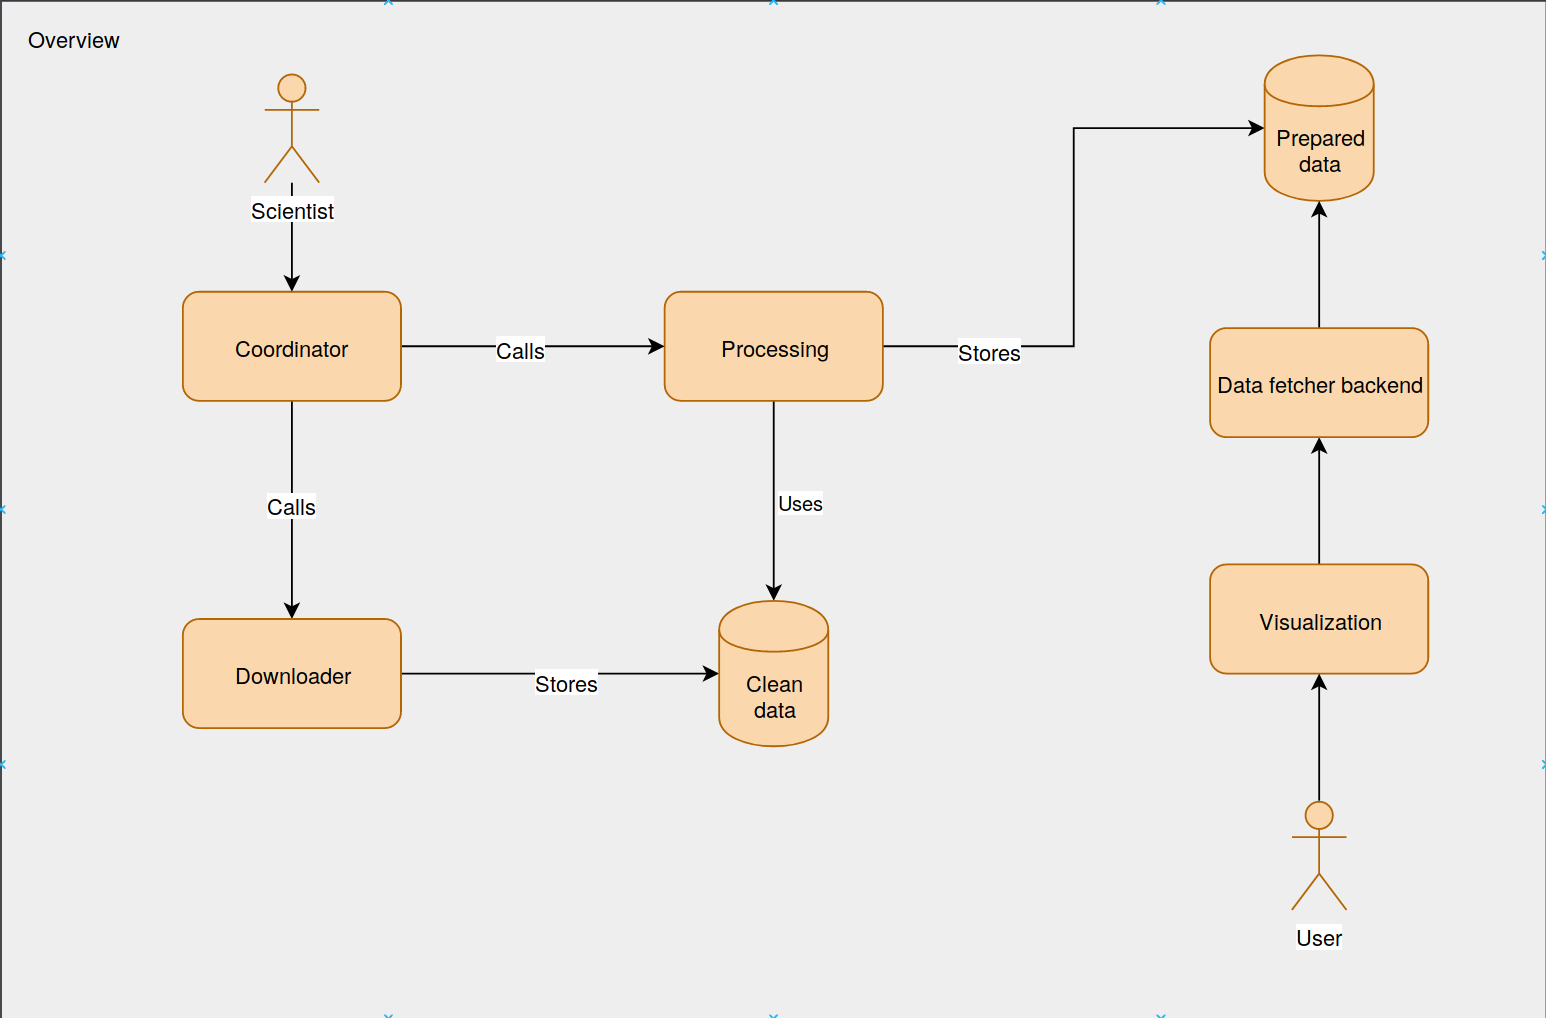
\includegraphics[width=10.5cm]{images/data_flow_overview.png}
		    	\caption{Data flow from database to \textit{k-means}}
		    	\label{fig:data_flow_pipeline}
		    \end{figure}
		
		    \vspace{1cm}
  	\subsection{Tools}
    % 	\subsubsection{Programming language: {\textit Scala}}
    
    
    \subsubsection{Database: {\textit MySQL}}
    \subsection{Downloader}
    \subsection{Coordinator}
    \subsection{API server}
%    \subsection{Repository}
    \subsection{User interface (Frontend)}
    
    \clearpage
    
    \section{Description of experimental research}
    \subsection{Data statistics}
    
   	Data statistics are calculated from data \gls{lrs_open} \acrshort{api} which was downloaded and saved to local database. Quite a big chunk data from 1997-2007 and 1990-1997 is missing due different information systems used at that time and other reasons. It was not migrated to current open data \acrshort{api}.
    
   	\noindent
    \begin{center}
    	\begin{tabular}{L{5cm} R{3cm}}
    		\multicolumn{2}{c}{}\\ 
    		\hline
    		Name & Count \\\hline
    		Term of offices & 8\\
    		Sessions & 101\\
    		Parliament members & 1207\\
    		Plenaries & 3977\\
    		Vote rows & 3933006\\
    		Votes & 28121\\
    		Agenda questions & 64243\\
    		Plenary questions (2012-) & 15108\\
    		Discussion events (2007-) & 361996\\
    		\hline
    	\end{tabular}
    	\captionof{table}{Statistics of downloaded data} \label{tab:data_statistics}
    \end{center}
    
    \hfill
    
    
   	\subsection{Experiments}
   	\subsubsection{MDS}
   	\subsubsection{Unsupervised learning: {\textit k-means} clusterization }
   	
   	\subsection{Results}
    
   
    \clearpage
    
    \bibliography{bibtex}{}
    \bibliographystyle{ieeetr}
        
    \clearpage
    
    \pagenumbering{roman}
      
	\appendix
	\section{Appendix}
    
    \end{document}